\documentclass[12pt,a4paper]{article}                                %%%
%%% Standard packages will be used by the Publisher:                 %%%
\usepackage{authblk,amsmath,amsfonts,amssymb,amsthm,graphicx}        %%%
\usepackage[textwidth=200mm,textheight=240mm]{geometry}              %%%
%                                                                    %%%
%%% Special commands:                                                %%%
\newcommand\Jcomm[2]{\par\medskip\noindent{\bfseries #1: } #2\par}   %%%
\newcommand\keywords[1]{\Jcomm{Keywords}{#1}}                        %%%
\newcommand\received[1]{\Jcomm{Received}{#1}}                        %%%
\newcommand\revised[1]{\Jcomm{Revised}{#1}}                          %%%
\newcommand\classification[1]{\Jcomm{MSC 2010}{#1}}                  %%%
\newcommand\acknowledgement[1]{\Jcomm{Acknowledgement}{#1}}          %%%
\newcommand\funding[1]{\Jcomm{Funding}{#1}}                          %%%
%                                                                    %%%
%%% Theorem styles:                                                  %%%
\numberwithin{equation}{section}                                     %%%
\theoremstyle{plain}                                                 %%%
  \newtheorem{theorem}{Theorem}[section]                             %%%
  \newtheorem{lemma}{Lemma}[section]                                 %%%
  \newtheorem{proposition}{Proposition}[section]                     %%%
\theoremstyle{definition}                                            %%%
  \newtheorem{definition}{Definition}[section]                       %%%
  \newtheorem{remark}{Remark}[section]                               %%%
  \newtheorem{corollary}{Corollary}[section]                         %%%
  \newtheorem{example}{Example}%[section]                            %%%
%                                                                    %%%
%%% Greek letters:                                                   %%%
\let\epsilon=\varepsilon                                             %%%                                               %%%
				                                                     %%
                                        %%%
%                                                                    %%%
\date{} %%% don't want date printed                                  %%%
\renewcommand\Authands{, }                                           %%%
%%% DO NOT EDIT BEFORE THIS LINE %%%%%%%%%%%%%%%%%%%%%%%%%%%%%%%%%%%%%%%

%%% Specify russian language and russian encoding if required
 \usepackage[T1,T2A]{fontenc}
 \usepackage[utf8]{inputenc} %%% specify cp866, cp1251, or koi8-r instead of utf8x if required
 \usepackage[english,russian]{babel}

\usepackage{graphics}      % standard graphics specifications
\usepackage{graphicx}      % alternative graphics specifications
\usepackage{caption}
\usepackage{subcaption}
\usepackage{amsmath}
\usepackage{cases}
\usepackage{multirow}
\usepackage{array}
\usepackage{booktabs}

\title{Вычисление скорости вылетания пули из ствола стрелкового оружия на основе уравнений Эйлера}
\author{Пережогин}
\begin{document}

\maketitle
%
%\begin{figure}[h!]
%      \centering
%      \includegraphics[width=1.0\textwidth]{povorot.jpg}
%      \caption{Графическое разъяснение происходящего.}
%\end{figure}

\section{Введение}
Оружейный патрон состоит из гильзы, капсуля и пули. 
В гильзе содержится порох, который способен гореть без участия кислорода.
Воспламенение пороха осуществляется за счет активирования капсуля.
В состав пороха входит горючая смесь (до 19 века, селитра)
и окислители (до 19 века, сера и углерод).
В результате сгорания пороха выделяются 
пороховые газы (CO2), которые обладают высоким давлением
и выталкивают пулю из ствола.

Предлагается рассмотреть две модели,
и сравнить скорость вылетания пули из ствола для них.
\begin{enumerate}
	\item Предположим, что пороховые газы 
	находятся в полном термодинамическом равновесии,
	а теплообмен между газом и окружающей средой отсутствует,
	т.е. расширение газа происходит адиабатически.
	Параметры модели следующие:
	
	$L_0$ и $S$ -- длина и поперечное сечение гильзы, задают начальный объем пороховых газов;
	$\varepsilon$ -- тепловая энергия, выделившаяся
	вследствие сгорания всего пороха;
	$\kappa$ -- масса порохового заряда;
	$\gamma$ -- показатель адиабаты;
	$m$ -- масса пули;
	$L_1$ -- длина ствола;
	площадь поперечного сечения ствола и гильзы совпадают.
	
	Скорость пули находится исходя из закона сохранения энергии
	для адиабатического процесса:
	внутренняя энергия газа передается пуле.
	
	\item Скорость пули может превышать скорость звука,
поэтому можно предположить, что пороховые газы не находятся в полном термодинамическом равновесии
в процессе вылетания пули из ствола, а наблюдается лишь 
локальное термодинамическое равновесие.
В этом случае состояние пороховых газов
задается в расширяющейся со временем расчетной области длины $L$, причем $L_0 \leq L \leq L_1$,
и используются одномерные уравнения Эйлера, см. \textit{[Годунов, Численное решение многомерных задач газовой динамики, Глава 2]}:
\begin{gather}
	\frac{\partial \rho}{\partial t} + \frac{\partial}{\partial x} \underbrace{(\rho u)}_{\text{поток массы}} = 0 \text{ -- закон сохранения массы}, \label{eq_1} \\
	\frac{\partial( \rho u )}{\partial t} + \frac{\partial }{\partial x} \underbrace{(\rho u^2)}_{\text{поток импульса}} = -
	\underbrace{\frac{\partial p}{\partial x}}_{\text{внешняя сила}} \text{ -- закон сохранения импульса}\\
	\frac{\partial (\rho E)}{\partial t} + \frac{\partial }{\partial x} \underbrace{(u \rho E)}_{\text{поток энергии}}= - 
	\underbrace{\frac{\partial (pu)}{\partial x}}_{\text{работа сил давления}}
	\text{ -- закон сохранения энергии}, \\
	p = (\gamma - 1) \rho e \text{ -- уравнение состояния идеального газа}, \label{eq_4}
\end{gather}
где $E = e + u^2/2$ -- полная энергия единицы массы газа, $u$ -- скорость,
$e$ -- внутренняя (тепловая) энергия единицы массы, $\rho$ -- плотность газа, 
$p$ -- давление, $\gamma$ -- показатель адиабаты.
Уравнение \eqref{eq_4} эквивалентно уравнению Менделеева-Клапейрона в наших переменных, см. \textit{[Уравнение 
состояния идеального газа, Википедия]}.

Также выписывается второй закон Ньютона для пули:
\begin{equation}
	m \frac{d v}{d t} = p(L)S, 
\end{equation}
где $m$ -- масса пули, $v$ -- скорость пули, 
$p(L)$ -- давление пороховых газов на границе с пулей,
$S$ -- площадь сечения ствола.
\end{enumerate}

\section{Параметры для некоторых видов стрелкового оружия}
Здесь предполагается, что теплота сгорания пороха составляет $900kcal/kg \approx 3.8kJ/g$,
что соответствует "Баллистическому пороху"{}, см. \textit{[Порох, Википедия]}.
Значение показателя адиабаты для всех видов оружия выбирается следующим:
\begin{equation}
	\gamma = 1.3.
\end{equation}
Таким показателем обладает углекислый газ (CO2) при температуре $20C^o$,
см. \textit{[Показатель адиабаты, Википедия]}.

\begin{enumerate}
	\item \textbf{Пистолет Макарова (ПМ) с патроном 9x18мм}.
	
	\begin{itemize}
		\item Длина гильзы, $L_0=18mm$.
		\item Поперечное сечение гильзы, $S=\pi (9mm)^2/4 \approx 64 mm^2$.
		\item Масса пули, $m=6g$.
		\item Масса порохового заряда $\kappa=0.25g$,
		следовательно, теплота сгорания пороха,
		
		
		$\varepsilon = 0.25 g \times  3.8kJ/g = 0.95kJ$.
		\item Длина ствола, $L_1 = 93mm$.
		\item Фактическая скорость пули для ПМ (измеренная), $315m/s$.
	\end{itemize}
	
	\item \textbf{Автомат Калашникова (АК-47) с патроном 7.62x39мм}.
	\begin{itemize}
		\item Длина гильзы, $L_0 = 39mm$.
		\item Поперечное сечение гильзы, $S=\pi (8mm)^2/4 \approx 50 mm^2$.
		\item Масса пули, $m=8g$.
		\item Масса порохового заряда $\kappa=1.75g$,
		следовательно, теплота сгорания пороха,
		
		
		$\varepsilon = 1.75 g \times  3.8kJ/g = 6.65kJ$.
		\item Длина ствола, $L_1 = 415mm$.
		\item Фактическая скорость пули для АК-47 (измеренная), $715m/s$.
	\end{itemize}
\end{enumerate}

\section{Скорости пули по 1 методу}
Термодинамическое состояние системы задается двумя параметрами. В нашем случае -- 
это начальная внутренняя энергия газа $U_0=\varepsilon$ и объем гильзы $V_0=S \cdot L_0$.
Уравнение для адиабатического процесса следующее, см. \textit{Адиабатический процесс, Википедия}:
\begin{equation}
	p \cdot V^\gamma = const.
\end{equation}
Модифицируем уравнение состояния \eqref{eq_4} к следующему виду:
\begin{equation}
	p = (\gamma-1) \frac{U}{V},
\end{equation}
где $U$ -- полная внутренняя энергия газа.
Комбинируя два последних уравнения получаем:
\begin{equation}
	U V^{\gamma-1} = const.
\end{equation}
Откуда:
\begin{equation}
	\frac{U_1}{U_0} = \left( \frac{V_0}{V_1} \right)^{\gamma-1} =  \left( \frac{L_0}{L_1} \right)^{\gamma-1}.
\end{equation}
Тогда изменение внутренней энергии газа равно кинетической энергии пули:
\begin{equation}
	K = U_0 - U_1 = \varepsilon \left(1 - \left(\frac{L_0}{L_1} \right)^{\gamma - 1} \right).
\end{equation}
КПД оружия не зависит от мощности заряда:
\begin{equation}
	\eta = \frac{K}{\varepsilon} \cdot 100\%.
\end{equation}

Наконец, скорость пули при выходе из ствола:
\begin{equation}
	v = \sqrt{\frac{2K}{m}}.
\end{equation}

Вычислим давление в начале и в конце:
\begin{itemize}
	\item $p_0 = (\gamma-1)\dfrac{\varepsilon}{S L_0}$,
	\item $p_1 = p_0 \left(\dfrac{L_0}{L_1} \right)^{\gamma}$.
\end{itemize}

\textit{Оценим} плотность газа в начальный момент времени.
Эта характеристика понадобится позже
при постановке начальных данных.
Предположим, что 
порох представлен \textit {только} селитрой ($KNO_3$) 
и при горении подчиняется химическому уравнению:
\begin{equation}
	2KNO_3 + 3 C + S \rightarrow K_2 S + N_2 + 3 CO_2,
\end{equation}
а пороховые газы представлены \textit{только} углекислым газом.
Молярная масса для селитры равна $M_{KNO_3} = 101g/mol$.
Тогда находим количество моль силитры:
\begin{equation}
	\nu_{KNO_3} = \kappa / M_{KNO_3}.
\end{equation}
Согласно химической формуле, количество моль
углекислого газа $\nu_{CO_2} = \frac{3}{2}\nu_{KNO_3} = \frac{3}{2}\kappa / M_{KNO_3}$.
Тогда плотность пороховых газов:
\begin{equation}
	\rho_0 = \nu_{CO_2} M_{CO_2} / V_0 = \frac{3}{2} \kappa \frac{M_{CO_2}}{M_{KNO_3}} / V_0,
\end{equation}
где молярная масса углекислого газа $M_{CO_2} = 44g/mol$.
\subsection{Вычисление на примерах}
\begin{enumerate}
	\item \textbf{Пистолет Макарова (ПМ)}.
	\begin{itemize}
		\item Кинетическая энергия пули, $K = 369.5J$.
		\item КПД, $\eta=38.9\%$.
		\item Давление в начальный момент, $p_0 = 2474$ атмосферы.
		\item Давление при вылете, $p_1=293$ атмосферы.
		\item Плотность пороховых газов в начале, $\rho_0=142 kg/m^3$.
		\item Скорость пули, $v=351m/s$.
		\item Измеренная скорость пули, $315m/s$.
	\end{itemize}
	
	\item \textbf{Автомат Калашникова (АК-47)}.
	\begin{itemize}
		\item Кинетическая энергия пули, $K = 3379J$.
		\item КПД, $\eta=50.8\%$.
		\item Давление в начальный момент, $p_0 = 10230$ атмосферы.
		\item Давление при вылете, $p_1=473$ атмосферы.
		\item Плотность пороховых газов в начале, $\rho_0 = 586 kg/m^3$.
		\item Скорость пули, $v=919m/s$.
		\item Измеренная скорость пули, $715m/s$.
	\end{itemize}
\end{enumerate}


Скорость пули достаточно близка к измеренной. Как видим, атмосферным давлением можно пренебречь.
Полученное нами давление пороховых газов при вылете лежит в разумных пределах.
В разных источниках приводятся значения $200-900$ атмосфер.
Давление в начальный момент, скорее всего, завышено, потому что 
в реальности пуля начинает двигаться еще до того, как прогорит весь порох.

\cleardoublepage

\section{Скорость пули по 2 методу}
В качестве динамических переменных (те, которые будут обновляться при решении уравнения) выберем следующие:
$\rho$, $\rho u$, $\rho E$.
В компактной форме уравнения Эйлера:
\begin{gather}
	\frac{\partial}{\partial t} 
	\begin{pmatrix}
		\rho \\
		\rho u \\
		\rho E
	\end{pmatrix}
	+  \frac{\partial}{\partial x}
	\begin{pmatrix}
		\rho u \\
		\rho u^2 + p \\
		\rho u E + pu
	\end{pmatrix}
	= 0,\\
	p = (\gamma - 1) \rho e,
\end{gather}
и помним, что
\begin{equation}
	E = e + u^2/2.
\end{equation}

Уравнение динамики пули:
\begin{gather}
	m \frac{d v}{d t} = p(L) S, \\
	\frac{d L}{d t} = v.
\end{gather}

Уравнения решаются в расширяющейся области $0<x<L(t)$,
поэтому сделаем замену координат $y = x / L(t)$,
$y\in[0,1]$.
Для некоторой переменной $\phi(x,t)$
частные производные преобразуются:
\begin{gather}
	\frac{\partial \phi(x,t)}{\partial t} = \frac{\partial \phi(L(t) y,t)}{\partial t}
	= \frac{v y}{L} \frac{\partial \phi(y,t)}{\partial y}  + \frac{\partial \phi(y,t)}{\partial t},\\
	\frac{\partial \phi}{\partial x} = \frac{1}{L} \frac{\partial \phi}{\partial y}.
\end{gather}

В новой горизонтальной координате уравнения Эйлера имеют вид:
\begin{gather}
	\frac{\partial}{\partial t} 
	\begin{pmatrix}
		\rho \\
		\rho u \\
		\rho E
	\end{pmatrix}
	+ \frac{v y}{L}
	\frac{\partial }{\partial y}
\begin{pmatrix}
		\rho \\
		\rho u \\
		\rho E
	\end{pmatrix}		
	+  \frac{1}{L} \frac{\partial}{\partial y}
	\begin{pmatrix}
		\rho u \\
		\rho u^2 + p \\
		\rho u E + pu
	\end{pmatrix}
	= 0,\\
	p = (\gamma - 1) \rho e, 
	\label{eq_5}
\end{gather}

Начальные условия следующие:
\begin{itemize}
	\item $\rho=\rho_0$. Проверить значения $\rho_0/2$, $2 \rho_0$.
	\item $\rho u=0$, т.к. скорость газа $u=0$
	\item $\rho E = \rho e = \dfrac{\varepsilon}{V_0} = \dfrac{\varepsilon}{S L_0}$
\end{itemize}

В качестве критериев устойчивости использовать максимум
из скорости звука
\begin{equation}
	c = \sqrt{\frac{\gamma p}{\rho}},
\end{equation}
и скорости газа.

\subsection{Постановка граничных условий}
Во-первых,
\begin{equation}
	u|_0=0, u|_1 = v
\end{equation}
и
\begin{equation}
	\frac{\partial p}{\partial y}|_0 = 0,
	\frac{\partial p}{\partial y}|_0 = 1.
\end{equation}
\paragraph{Сохранение массы}
Масса газа должна сохраняться, значит
\begin{equation}
	\int_0^{L(t)} \rho(x,t) dx = L(t) \int_0^1 \rho(y,t) dy = const. 
\end{equation}
Тогда:
\begin{equation}
	\frac{d L}{d t} \int_0^1 \rho(y,t) dy + L(t)  \int_0^1 \frac{\partial \rho}{\partial t} dy = 0.
\end{equation}
Подставляя в это равенство закон сохранения массы (верхнее уравнение из \eqref{eq_5}),
применяя гран условия $u(0,t) = 0, u(1,t) = v$,
получаем:
\begin{equation}
	v \int_0^1 \rho dy - v \int_0^1 y \frac{\partial \rho}{\partial y} dy - \int_0^1 \frac{\partial \rho u}{\partial y} dy =
	2 v \int_0^1 \rho dy  - 2 (u \rho)|_1 = 0.
\end{equation}
Следовательно, 
\begin{equation}
	(u \rho)|_0=0, \\
	(u \rho)|_1= v\int_0^1 \rho dy.
\end{equation}

\paragraph{Сохранение импульса}
Предполагаем, что полный импульс газа может изменяться
только вследствие
взаимодействия с левой и правой стенками
посредством давления.
Потребуем этого.
Полный импульс газа:
\begin{equation}
	L(t) \int_0^1 \rho u dy  \rightarrow  \frac{d L}{d t} \int_0^1 \rho u dy
	+ L(t) \int_0^1 \frac{\partial \rho u}{\partial t} dy.
\end{equation}
Подставляем в это равенство уравнение движения:
\begin{equation}
	v \int_0^1 \rho u dy - v \int_0^1 y \frac{\partial \rho u}{\partial y} dy-
	\int_0^1 \frac{\partial}{\partial y}(\rho u^2 + p) dy =
	2v \int_0^1 \rho u dy - 2 (\rho u^2)|_1 - p|_0^1.
\end{equation}
Откуда:
\begin{equation}
	(\rho u^2)|_0 = 0, 
	(\rho u^2)|_1 = v \int_0^1 \rho u dy.
\end{equation}

\paragraph{Сохранение энергии}
Потребуем, чтобы полная энергия газа менялась только следствие работы,
совершаемой над пулей.
Энергия:
\begin{equation}
	L(t) \int_0^1 \rho E dy \rightarrow \frac{d L}{d t} \int_0^1 \rho E dy
	+ L(t) \int_0^1 \frac{\partial \rho E}{\partial t} dy.
\end{equation}
Тогда:
\begin{equation}
	v \int_0^1 \rho E dy - v \int_0^1 y \frac{\partial \rho E}{\partial y} dy - \int_0^1 \frac{\partial }{\partial y} (\rho u E + p u) dy
	= 2 v \int_0^1 \rho E dy - 2 (\rho u E) |_1 - v p|_1
\end{equation}
Гран условия:
\begin{equation}
	(\rho u E)|_0 = 0,
	(\rho u E)|_1 = v \int_0^1 \rho E dy.
\end{equation}

\paragraph{Гран условия в связи со сменой координат}
Заметим, 
что для оператора
$\frac{v y}{L}
	\frac{\partial }{\partial y}
\begin{pmatrix}
		\rho \\
		\rho u \\
		\rho E
	\end{pmatrix}		$
постановка гран условий не требуется. В самом деле,
характеристики
для этого оператора 
выходят из левого конца области.
Но в левой граничной точке скорость переноса $(vy/L)$
равна нулю.

\begin{figure}[h!]
      \centering
      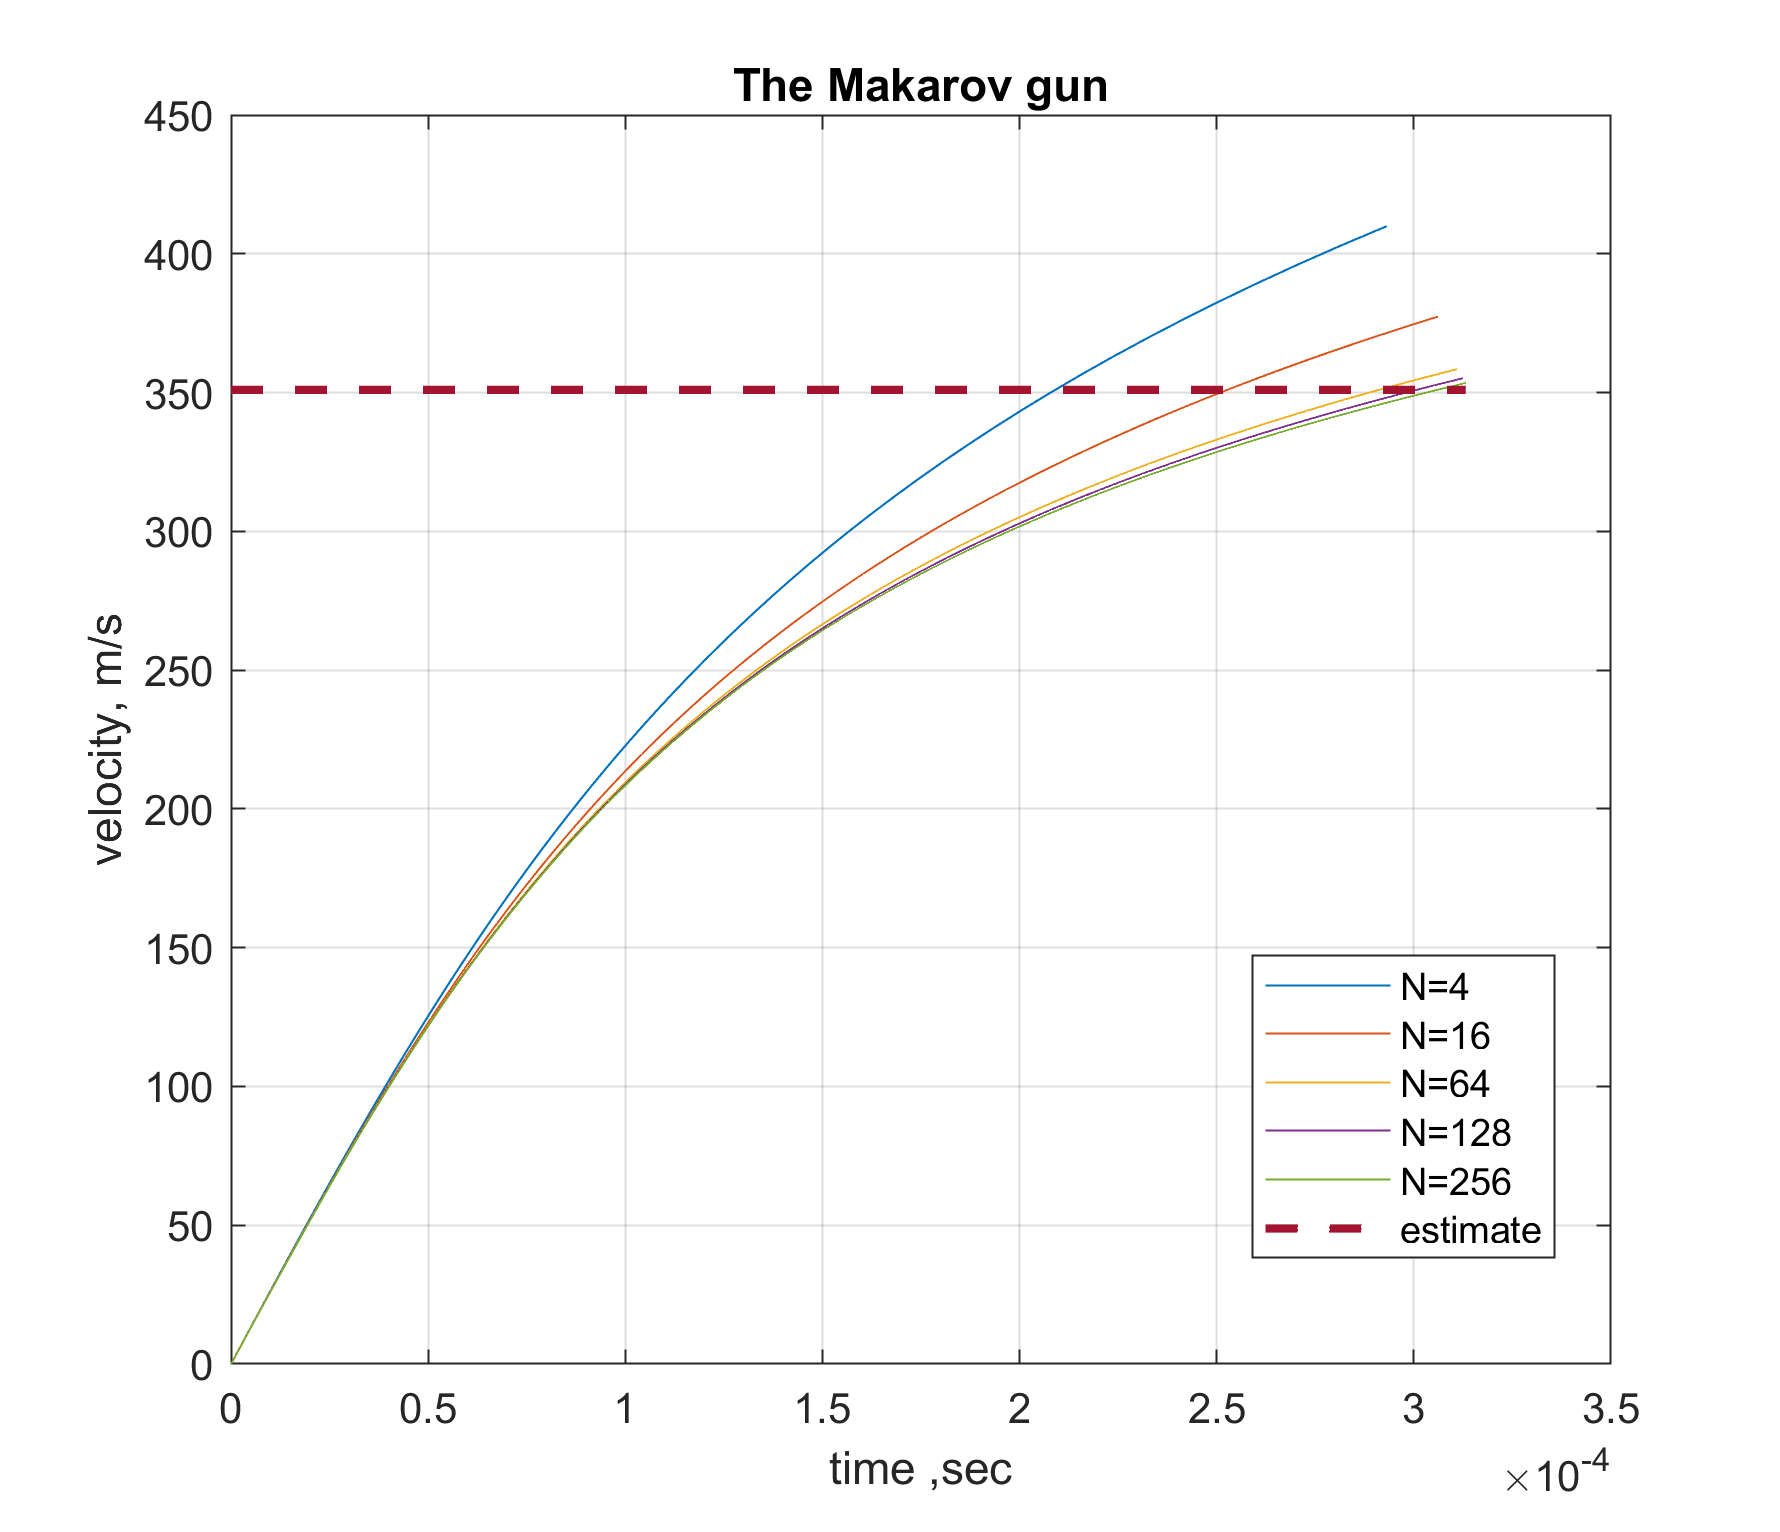
\includegraphics[width=0.5\textwidth]{makarov.png}
      \caption{Пример расчета для пистолета Макарова при числе узлов сетки $N$.}
\end{figure}

\subsection{Переход к консервативным переменным}
Перейдем к новым переменным
\begin{gather}
	\widehat{\rho} = L(t) \rho, \\
	\widehat{\rho u} = L(t) \rho u, \\
	\widehat{\rho E} = L(t) \rho E.
\end{gather}
Тогда закон сохранения массы газа:
\begin{equation}
	\int \widehat{\rho} dy = const,
\end{equation}
а также импульс и энергия могут меняться только за счет давления на границах области:
\begin{gather}
	\frac{d}{dt} \int \widehat{\rho u} dy = F(p), \\
	\frac{d}{dt} \int \widehat{\rho E} dy = G(p). \\
\end{gather}

Перепишем уравнения движения \eqref{eq_5}
в новых переменных:
\begin{gather}
	\frac{\partial}{\partial t} 
	\begin{pmatrix}
		\widehat{\rho} \\
		\widehat{\rho u} \\
		\widehat{\rho E}
	\end{pmatrix}
	-\frac{2 v}{L} 
		\begin{pmatrix}
		\widehat{\rho} \\
		\widehat{\rho u} \\
		\widehat{\rho E}
	\end{pmatrix}
	+  \frac{1}{L} \frac{\partial}{\partial y}
	\begin{pmatrix}
		\widehat{\rho u} + \widehat{\rho} v y \\
		\rho u^2 + p \\
		\rho u E + pu
	\end{pmatrix}
	= 0,\\
	p = (\gamma - 1) \rho e, 
\end{gather}
\end{document}